 Use the secant method to solve the bvp
% \begin{equation*}
% \begin{split}
% y'' &= -4y -9\sin(x), \quad x \in [0,3\pi/4],\\
% y(0) &= 1, \\
% y(3\pi/4) &=-\frac{1+3\sqrt{2}}{2}.
% \end{split}
% \end{equation*}
% When you code the secant method, be sure to include a maximum number of iterations, as well as an appropriate stopping criteria.
% For example, if $|y(b,t_n)-\beta|<10^{-8},$ you have likely found a solution.
% 
Appropriately defined initial value problems will usually have a unique solution.
Boundary value problems are not so straightforward; they may have no solution or they may have several.
You may have to determine which solution is physically interesting.
The following bvp has at least two solutions.
Using the secant method, find both numerical solutions and their initial slopes.
(Their plots are given in Figure \ref{prob:shooting1}.)
What initial values $t_0, t_1$ did you use to find them?
\begin{equation*}
\begin{split}
y'' &= -4y -9\sin(x), \,\, x \in [0,\pi],\\
y(0) &= 1, \\
y(\pi) &=1.
\end{split}
\end{equation*}

\begin{figure}[H]
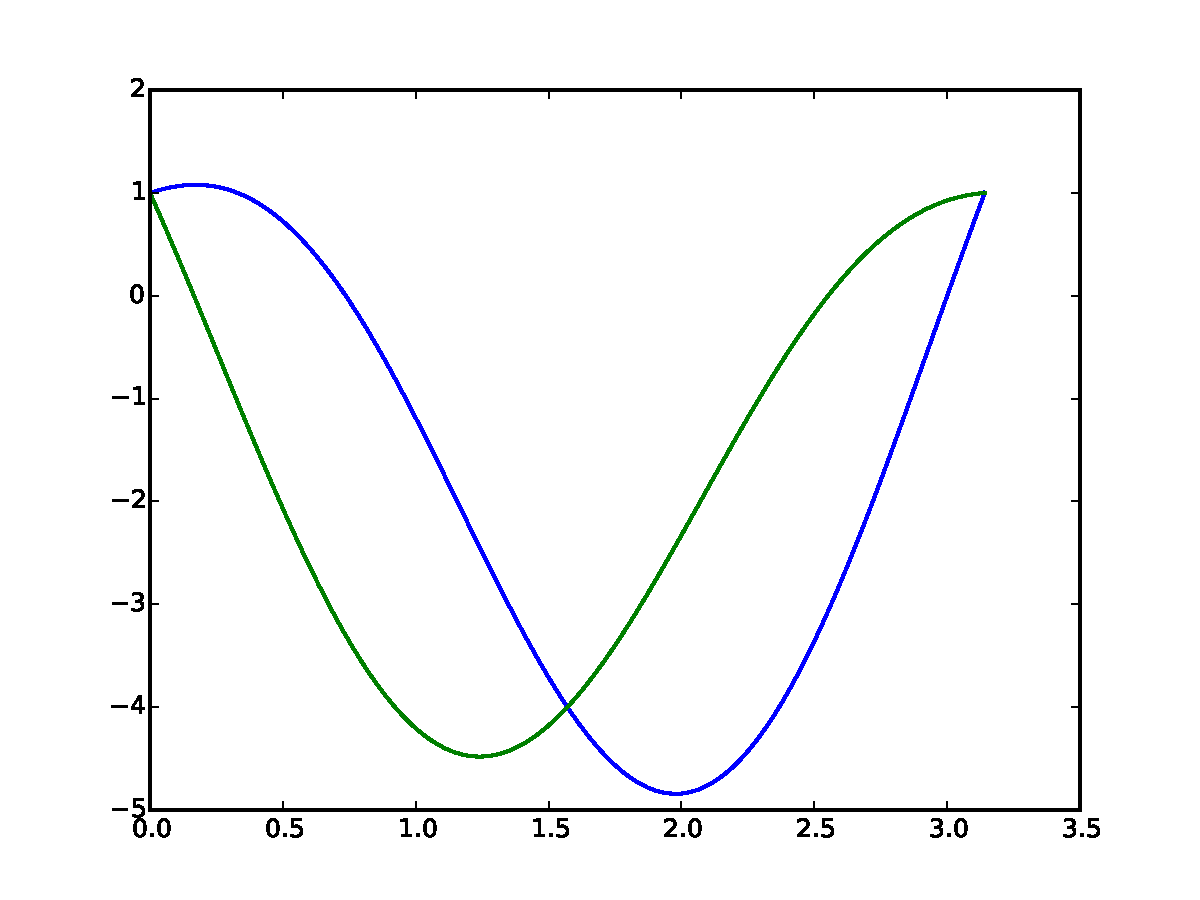
\includegraphics[width=\textwidth]{Fig1.pdf}
\caption{Two solutions of $y'' = -4y -9\sin(x),$ both satisfying the boundary conditions $y(0) = y(\pi) = 1.$}
\label{prob:shooting1}
\end{figure}

Use Newton's method to solve the BVP
\begin{equation*}
\begin{split}
y'' &= 3 + \frac{2y}{x^2}, \,\, x \in [1,e],\\
y(1) &= 6, \\
y(e) &= e^2 + 6/e.
\end{split}
\end{equation*}
Plot your solution.
(Compare with Figure \ref{prob:shooting2}.)
What is an appropriate initial guess?

Hint: Update the ode() function from the previous problem to solve for $y$, $y'$, $z$, $z'$ simultaneously.
This can be done by first rewriting the equations for $y"$ and $z"$ as a system of first order differential equations.

\begin{figure}[H]
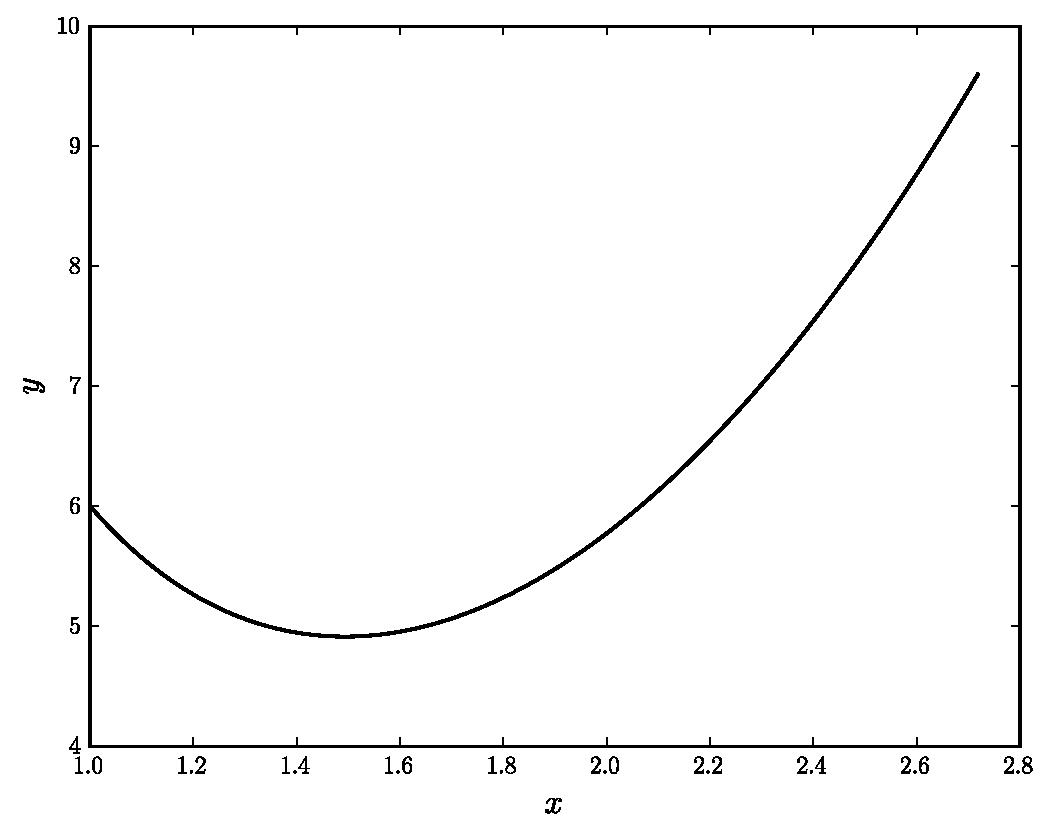
\includegraphics[width=\textwidth]{Fig2.pdf}
\caption{The solution of  $y'' = 3 + 2y/x^2,$ satisfying the boundary conditions $y(1) = 6$, $ y(e) =  e^2 + 6/e$.}
\label{prob:shooting2}
\end{figure}

Suppose a projectile is fired from a cannon with velocity $45\text{ m/s}^2$.
At what angle $\theta(0)$ should it be fired to land at a distance of $195\text{ m}$?

There should be two initial angles $\theta(0)$ that produce a solution for this bvp.
Use the secant method to numerically compute and then plot both trajectories.
\begin{align}
	\label{eqn:cannon_shooting}
	\begin{split}
\frac{dy}{dx} &= \tan {\theta} ,\\
\frac{dv}{dx} &= -\frac{g \sin{\theta} + \mu v^2}{v \cos{\theta}},\\
\frac{d\theta}{dx} &= -\frac{g}{v^2},\\
y(0)&= y(195) = 0,\\
v(0) &= 45 \text{ m/s}^2
	\end{split}
\end{align}
($g = 9.8067\text{ m/s}^2$.)
Find both solutions for this boundary value problem when $\mu = .0003$.
Compare with the solutions when $\mu = 0.$
Their graphs are given in Figure \ref{fig:shooting_cannon_comparison2}.

Hint: This is a system of three first order differential equations, and so our secant method requires a slight modification.
Keeping in mind that the unknown initial condition is $\theta(0)$, not $y'(0)$, define an appropriate function $h(t)$.
